{\centering
\section{Calibrazione del magnete}
}
\medskip
{\color{gray}\hrule}
\medskip
Lo scopo di questa parte è calibrare il magnete, ovvero determinare la dipendenza del campo magnetico, generato tra le espansioni polari, dalla corrente iniettata nelle bobine. Infatti, la grandezza controllata sperimentalmente è la corrente $I$, mentre la separazione delle righe spettrali dipende dall’intensità del campo magnetico applicato $B$. È quindi necessario determinare la relazione $B(I)$ per poter associare a ciascun valore di corrente il corrispondente valore di campo magnetico e successivamente ricavare una stima del magnetone di Bohr.

Si realizza dunque il circuito di alimentazione del magnete, connettendo un generatore di tensione in parallelo a un condensatore di sicurezza e a un amperometro\footnote{Modello PeakTech 3335 DMM.} per la misura della corrente, collegato a sua volta in serie alle due bobine. Per la misura del campo magnetico si utilizza un teslametro\footnote{Modello Extech SDL900.}.

\subsection{Uniformità del campo magnetico tra le espansioni polari}

Prima di eseguire le misure di $B(I)$, si valuta il grado di uniformità del campo magnetico tra le espansioni polari nella regione attorno all’asse centrale, cioè nell’area della finestra di emissione della lampada. Poiché la sorgente luminosa non è puntiforme, diverse porzioni della lampada possono essere soggette a valori leggermente diversi del campo magnetico: tale non uniformità comporterebbe una diversa separazione delle componenti spettrali a seconda delle zone della sorgente, introducendo un’ulteriore incertezza nella misura.

Dopo aver impostato nel circuito del magnete una corrente di circa $2.3$A, si effettuano 7 misure di $B$, spostando il teslametro sulle superfici dei piani perpendicolari e paralleli al campo magnetico (riportate in appendice \ref{sec:unif}).\\
Si utlizza come incertezza sulle misure di $B$ il valore minimo la
semidispersione massima di queste misure
$$\sigma_{B,min,I=2.3 A}= 15.0 \text{mT}$$
e l'incertezza del teslametro.

Anche nella parte della stima del magnetone di Bohr si è adottata $\sigma_{B,min}$ come incertezza minima sui valori di $B$.
\subsection{Relazione di calibrazione $\mathbf{B(I)}$}
A questo punto si procede alla stima della relazione di calibrazione $B(I)$: si misura
$B$ sull'asse centrale delle espansioni polari variando la corrente iniettata nelle bobine a passi di 1A, da $0$A a $10$A e da $10$A a $0$A, ripetendo tale procedimento di misura una seconda volta (tutti i dati sono riportati nella sezione \ref{sec:B_I} in Appendice).\\
Si ottengono 4 set di dati, due di salita e due di discesa, su cui si effettuano 4 fit lineari.\\
I risultati si riportano di seguito.
\begin{multicols}{2}
\begin{figure}[H]
    \centering
    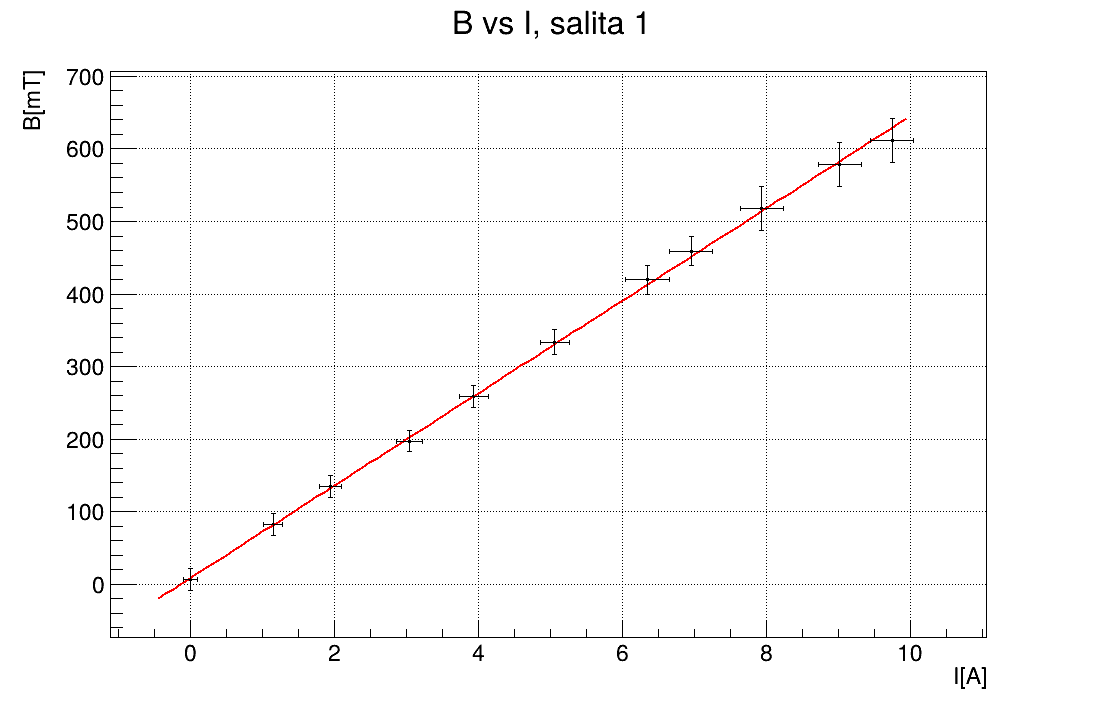
\includegraphics[width=\linewidth]{calibrazione/salita1.png}
    \caption{\footnotesize Coppie di valori ($B_i$,$I_i$) per la prima salita e fit lineare $y=mx+q$ con parametri\\ $m=(64\pm2)\text{mT/A}$, $q=(8\pm11)\text{mT}$, $\chi^2=0.52$ e d.o.f.=$9$.}
\end{figure}

\begin{figure}[H]
    \centering
    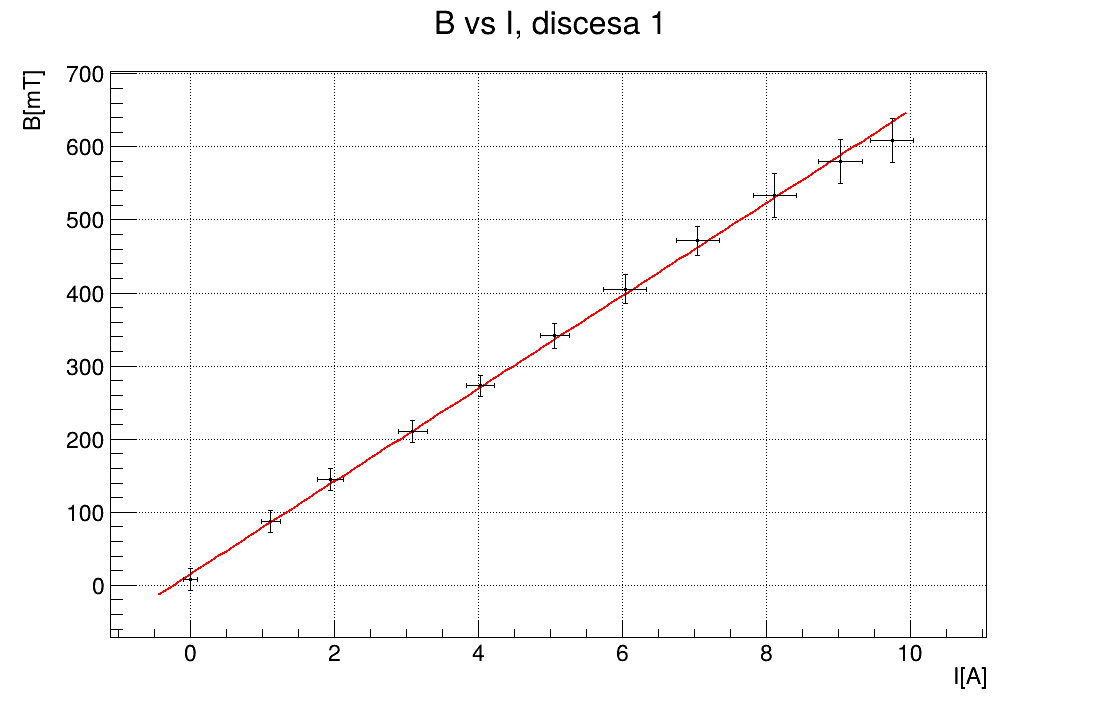
\includegraphics[width=\linewidth]{calibrazione/discesa1.png}
    \caption{\footnotesize Coppie di valori ($B_i$,$I_i$) per la prima discesa e fit lineare
    $y=mx+q$ con parametri\\ $m=(63\pm2)\text{mT/A}$, $q=(15\pm11)\text{mT}$, $\chi^2=1.1$ e d.o.f.=$9$. }
\end{figure}
\end{multicols}
\begin{multicols}{2}
\begin{figure}[H]
    \centering
    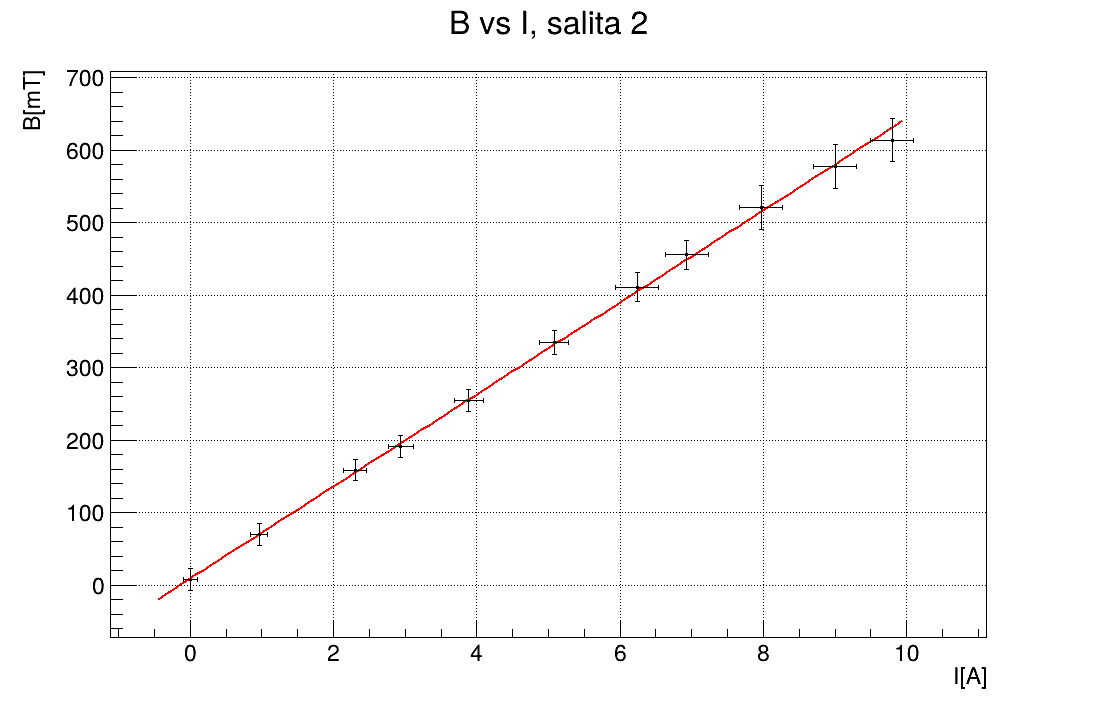
\includegraphics[width=\linewidth]{calibrazione/salita2.png}
    \caption{\footnotesize Coppie di valori ($B_i$,$I_i$) per la seconda salita e fit lineare $y=mx+q$ con parametri\\ $m=(63\pm2)\text{mT/A}$, $q=(10\pm10)\text{mT}$, $\chi^2=0.51$ e d.o.f.=$9$.}
\end{figure}
\begin{figure}[H]
    \centering
    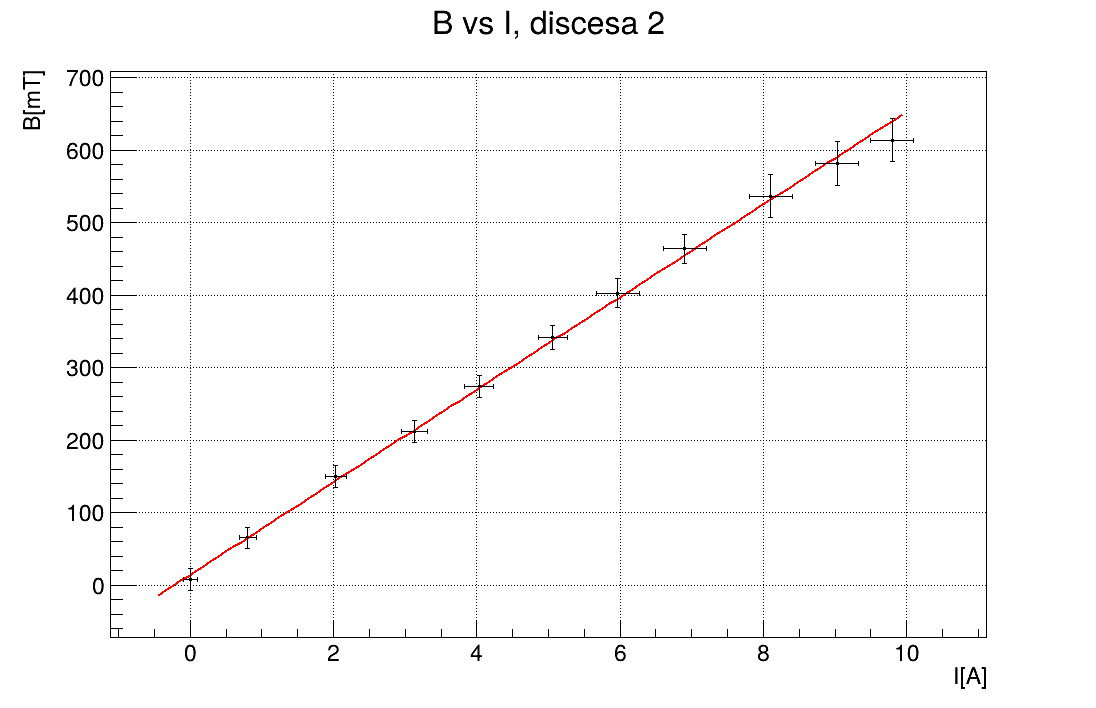
\includegraphics[width=\linewidth]{calibrazione/discesa2.png}
    \caption{\footnotesize Coppie di valori ($B_i$,$I_i$) per la seconda discesa e fit lineare $y=mx+q$ con parametri\\ $m=(64\pm2)mT/A$, $q=(14\pm10)mT$,$\chi^2=1.15$ e d.o.f.=$9$.}
\end{figure}
\end{multicols}
Per ricavare la curva di calibrazione si sono prima mediati separatamente i parametri fittati
per discesa e salita e si sono poi confrontate queste medie tra di loro:
sia i coefficienti angolari, sia i termini noti risultano statisticamente compatibili e se ne prende la media pesata.\\
La curva di calibrazione è dunque
\begin{equation}
    B(I) = (63.9\pm1.2)\text{mT/A}\cdot I + (12\pm5)\text{mT}
    \label{eq:cal_magn}
\end{equation}
Dal fatto che non solo i coefficienti angolari, ma anche i termini noti risultino
statisticamente compatibili si può affermare che il ferromagnete utilizzato è
abbastanza dolce da poter trascurare gli effetti del ciclo di isteresi, in quanto essi
non vengono risolti dal setup sperimentale.
